\documentclass[1p]{elsarticle_modified}
%\bibliographystyle{elsarticle-num}

%\usepackage[colorlinks]{hyperref}
%\usepackage{abbrmath_seonhwa} %\Abb, \Ascr, \Acal ,\Abf, \Afrak
\usepackage{amsfonts}
\usepackage{amssymb}
\usepackage{amsmath}
\usepackage{amsthm}
\usepackage{scalefnt}
\usepackage{amsbsy}
\usepackage{kotex}
\usepackage{caption}
\usepackage{subfig}
\usepackage{color}
\usepackage{graphicx}
\usepackage{xcolor} %% white, black, red, green, blue, cyan, magenta, yellow
\usepackage{float}
\usepackage{setspace}
\usepackage{hyperref}

\usepackage{tikz}
\usetikzlibrary{arrows}

\usepackage{multirow}
\usepackage{array} % fixed length table
\usepackage{hhline}

%%%%%%%%%%%%%%%%%%%%%
\makeatletter
\renewcommand*\env@matrix[1][\arraystretch]{%
	\edef\arraystretch{#1}%
	\hskip -\arraycolsep
	\let\@ifnextchar\new@ifnextchar
	\array{*\c@MaxMatrixCols c}}
\makeatother %https://tex.stackexchange.com/questions/14071/how-can-i-increase-the-line-spacing-in-a-matrix
%%%%%%%%%%%%%%%

\usepackage[normalem]{ulem}

\newcommand{\msout}[1]{\ifmmode\text{\sout{\ensuremath{#1}}}\else\sout{#1}\fi}
%SOURCE: \msout is \stkout macro in https://tex.stackexchange.com/questions/20609/strikeout-in-math-mode

\newcommand{\cancel}[1]{
	\ifmmode
	{\color{red}\msout{#1}}
	\else
	{\color{red}\sout{#1}}
	\fi
}

\newcommand{\add}[1]{
	{\color{blue}\uwave{#1}}
}

\newcommand{\replace}[2]{
	\ifmmode
	{\color{red}\msout{#1}}{\color{blue}\uwave{#2}}
	\else
	{\color{red}\sout{#1}}{\color{blue}\uwave{#2}}
	\fi
}

\newcommand{\Sol}{\mathcal{S}} %segment
\newcommand{\D}{D} %diagram
\newcommand{\A}{\mathcal{A}} %arc


%%%%%%%%%%%%%%%%%%%%%%%%%%%%%5 test

\def\sl{\operatorname{\textup{SL}}(2,\Cbb)}
\def\psl{\operatorname{\textup{PSL}}(2,\Cbb)}
\def\quan{\mkern 1mu \triangleright \mkern 1mu}

\theoremstyle{definition}
\newtheorem{thm}{Theorem}[section]
\newtheorem{prop}[thm]{Proposition}
\newtheorem{lem}[thm]{Lemma}
\newtheorem{ques}[thm]{Question}
\newtheorem{cor}[thm]{Corollary}
\newtheorem{defn}[thm]{Definition}
\newtheorem{exam}[thm]{Example}
\newtheorem{rmk}[thm]{Remark}
\newtheorem{alg}[thm]{Algorithm}

\newcommand{\I}{\sqrt{-1}}
\begin{document}

%\begin{frontmatter}
%
%\title{Boundary parabolic representations of knots up to 8 crossings}
%
%%% Group authors per affiliation:
%\author{Yunhi Cho} 
%\address{Department of Mathematics, University of Seoul, Seoul, Korea}
%\ead{yhcho@uos.ac.kr}
%
%
%\author{Seonhwa Kim} %\fnref{s_kim}}
%\address{Center for Geometry and Physics, Institute for Basic Science, Pohang, 37673, Korea}
%\ead{ryeona17@ibs.re.kr}
%
%\author{Hyuk Kim}
%\address{Department of Mathematical Sciences, Seoul National University, Seoul 08826, Korea}
%\ead{hyukkim@snu.ac.kr}
%
%\author{Seokbeom Yoon}
%\address{Department of Mathematical Sciences, Seoul National University, Seoul, 08826,  Korea}
%\ead{sbyoon15@snu.ac.kr}
%
%\begin{abstract}
%We find all boundary parabolic representation of knots up to 8 crossings.
%
%\end{abstract}
%\begin{keyword}
%    \MSC[2010] 57M25 
%\end{keyword}
%
%\end{frontmatter}

%\linenumbers
%\tableofcontents
%
\newcommand\colored[1]{\textcolor{white}{\rule[-0.35ex]{0.8em}{1.4ex}}\kern-0.8em\color{red} #1}%
%\newcommand\colored[1]{\textcolor{white}{ #1}\kern-2.17ex	\textcolor{white}{ #1}\kern-1.81ex	\textcolor{white}{ #1}\kern-2.15ex\color{red}#1	}

{\Large $\underline{12n_{0559}~(K12n_{0559})}$}

\setlength{\tabcolsep}{10pt}
\renewcommand{\arraystretch}{1.6}
\vspace{1cm}\begin{tabular}{m{100pt}>{\centering\arraybackslash}m{274pt}}
\multirow{5}{120pt}{
	\centering
	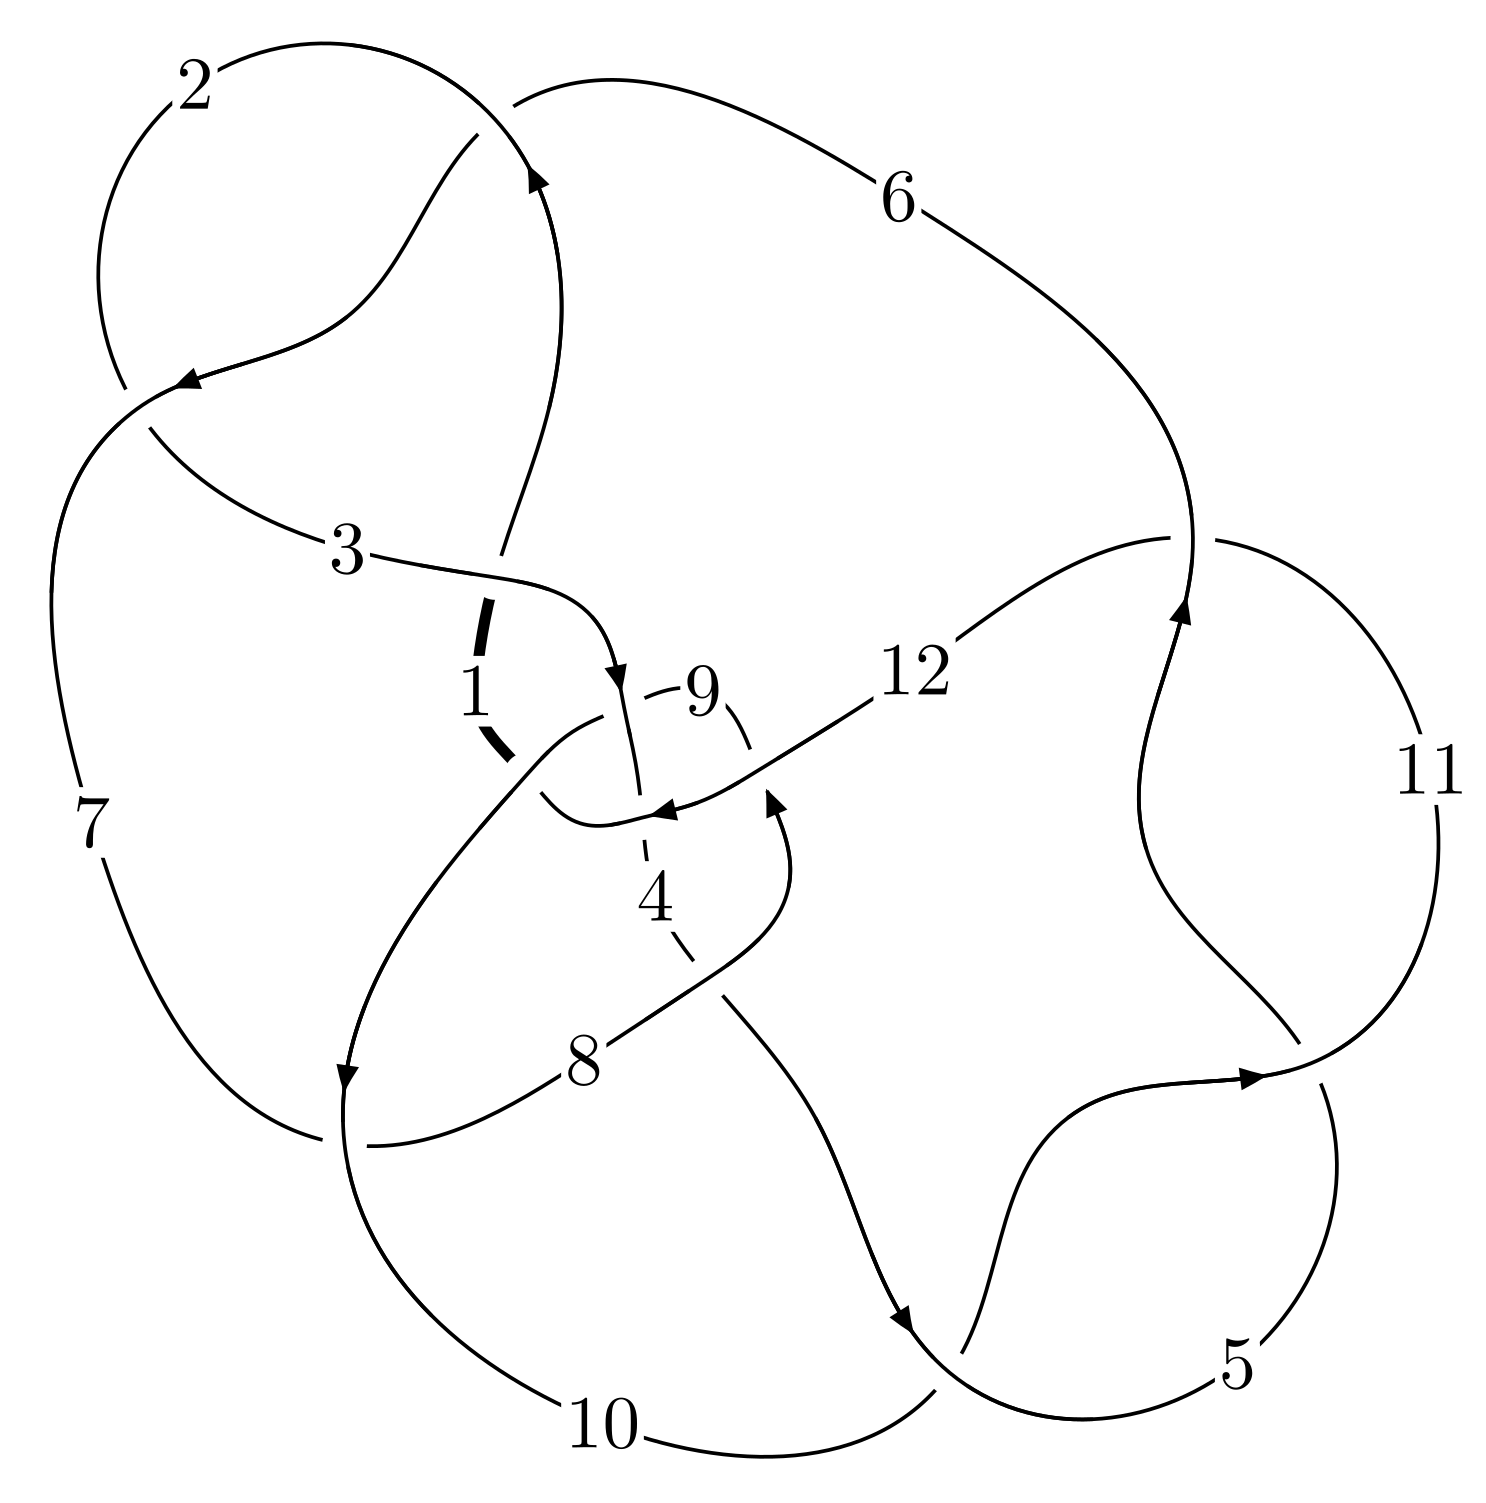
\includegraphics[width=112pt]{../../../GIT/diagram.site/Diagrams/png/2648_12n_0559.png}\\
\ \ \ A knot diagram\footnotemark}&
\allowdisplaybreaks
\textbf{Linearized knot diagam} \\
\cline{2-2}
 &
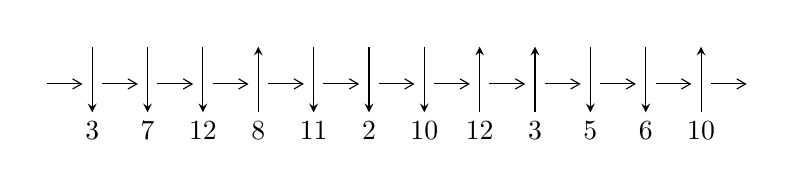
\begin{tikzpicture}[x=20pt, y=17pt]
	% nodes
	\node (C0) at (0, 0) {};
	\node (C1) at (1, 0) {};
	\node (C1U) at (1, +1) {};
	\node (C1D) at (1, -1) {3};

	\node (C2) at (2, 0) {};
	\node (C2U) at (2, +1) {};
	\node (C2D) at (2, -1) {7};

	\node (C3) at (3, 0) {};
	\node (C3U) at (3, +1) {};
	\node (C3D) at (3, -1) {12};

	\node (C4) at (4, 0) {};
	\node (C4U) at (4, +1) {};
	\node (C4D) at (4, -1) {8};

	\node (C5) at (5, 0) {};
	\node (C5U) at (5, +1) {};
	\node (C5D) at (5, -1) {11};

	\node (C6) at (6, 0) {};
	\node (C6U) at (6, +1) {};
	\node (C6D) at (6, -1) {2};

	\node (C7) at (7, 0) {};
	\node (C7U) at (7, +1) {};
	\node (C7D) at (7, -1) {10};

	\node (C8) at (8, 0) {};
	\node (C8U) at (8, +1) {};
	\node (C8D) at (8, -1) {12};

	\node (C9) at (9, 0) {};
	\node (C9U) at (9, +1) {};
	\node (C9D) at (9, -1) {3};

	\node (C10) at (10, 0) {};
	\node (C10U) at (10, +1) {};
	\node (C10D) at (10, -1) {5};

	\node (C11) at (11, 0) {};
	\node (C11U) at (11, +1) {};
	\node (C11D) at (11, -1) {6};

	\node (C12) at (12, 0) {};
	\node (C12U) at (12, +1) {};
	\node (C12D) at (12, -1) {10};
	\node (C13) at (13, 0) {};

	% arrows
	\draw[->,>={angle 60}]
	(C0) edge (C1) (C1) edge (C2) (C2) edge (C3) (C3) edge (C4) (C4) edge (C5) (C5) edge (C6) (C6) edge (C7) (C7) edge (C8) (C8) edge (C9) (C9) edge (C10) (C10) edge (C11) (C11) edge (C12) (C12) edge (C13) ;	\draw[->,>=stealth]
	(C1U) edge (C1D) (C2U) edge (C2D) (C3U) edge (C3D) (C4D) edge (C4U) (C5U) edge (C5D) (C6U) edge (C6D) (C7U) edge (C7D) (C8D) edge (C8U) (C9D) edge (C9U) (C10U) edge (C10D) (C11U) edge (C11D) (C12D) edge (C12U) ;
	\end{tikzpicture} \\
\hhline{~~} \\& 
\textbf{Solving Sequence} \\ \cline{2-2} 
 &
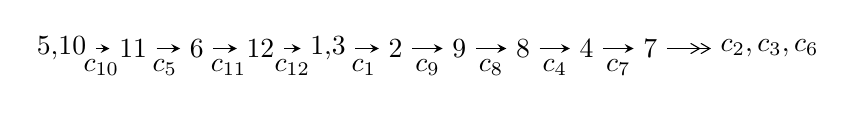
\begin{tikzpicture}[x=23pt, y=7pt]
	% node
	\node (A0) at (-1/8, 0) {5,10};
	\node (A1) at (1, 0) {11};
	\node (A2) at (2, 0) {6};
	\node (A3) at (3, 0) {12};
	\node (A4) at (65/16, 0) {1,3};
	\node (A5) at (41/8, 0) {2};
	\node (A6) at (49/8, 0) {9};
	\node (A7) at (57/8, 0) {8};
	\node (A8) at (65/8, 0) {4};
	\node (A9) at (73/8, 0) {7};
	\node (C1) at (1/2, -1) {$c_{10}$};
	\node (C2) at (3/2, -1) {$c_{5}$};
	\node (C3) at (5/2, -1) {$c_{11}$};
	\node (C4) at (7/2, -1) {$c_{12}$};
	\node (C5) at (37/8, -1) {$c_{1}$};
	\node (C6) at (45/8, -1) {$c_{9}$};
	\node (C7) at (53/8, -1) {$c_{8}$};
	\node (C8) at (61/8, -1) {$c_{4}$};
	\node (C9) at (69/8, -1) {$c_{7}$};
	\node (A10) at (11, 0) {$c_{2},c_{3},c_{6}$};

	% edge
	\draw[->,>=stealth]	
	(A0) edge (A1) (A1) edge (A2) (A2) edge (A3) (A3) edge (A4) (A4) edge (A5) (A5) edge (A6) (A6) edge (A7) (A7) edge (A8) (A8) edge (A9) ;
	\draw[->>,>={angle 60}]	
	(A9) edge (A10);
\end{tikzpicture} \\ 

\end{tabular} \\

\footnotetext{
The image of knot diagram is generated by the software ``\textbf{Draw programme}" developed by Andrew Bartholomew(\url{http://www.layer8.co.uk/maths/draw/index.htm\#Running-draw}), where we modified some parts for our purpose(\url{https://github.com/CATsTAILs/LinksPainter}).
}\phantom \\ \newline 
\centering \textbf{Ideals for irreducible components\footnotemark of $X_{\text{par}}$} 
 
\begin{align*}
I^u_{1}&=\langle 
-2.74895\times10^{16} u^{37}+2.53324\times10^{16} u^{36}+\cdots+4.11981\times10^{16} b-1.42189\times10^{17},\\
\phantom{I^u_{1}}&\phantom{= \langle  }-1.62383\times10^{17} u^{37}+1.68076\times10^{17} u^{36}+\cdots+8.23961\times10^{16} a-1.06430\times10^{18},\;u^{38}- u^{37}+\cdots+7 u-1\rangle \\
I^u_{2}&=\langle 
- u^5+2 u^3+b- u,\;- u^5-2 u^3 a+2 u^4+u^2 a+2 u^3+a^2+2 a u-3 u^2- a- u,\;u^6-3 u^4+2 u^2+1\rangle \\
\\
\end{align*}
\raggedright * 2 irreducible components of $\dim_{\mathbb{C}}=0$, with total 50 representations.\\
\footnotetext{All coefficients of polynomials are rational numbers. But the coefficients are sometimes approximated in decimal forms when there is not enough margin.}
\newpage
\renewcommand{\arraystretch}{1}
\centering \section*{I. $I^u_{1}= \langle -2.75\times10^{16} u^{37}+2.53\times10^{16} u^{36}+\cdots+4.12\times10^{16} b-1.42\times10^{17},\;-1.62\times10^{17} u^{37}+1.68\times10^{17} u^{36}+\cdots+8.24\times10^{16} a-1.06\times10^{18},\;u^{38}- u^{37}+\cdots+7 u-1 \rangle$}
\flushleft \textbf{(i) Arc colorings}\\
\begin{tabular}{m{7pt} m{180pt} m{7pt} m{180pt} }
\flushright $a_{5}=$&$\begin{pmatrix}0\\u\end{pmatrix}$ \\
\flushright $a_{10}=$&$\begin{pmatrix}1\\0\end{pmatrix}$ \\
\flushright $a_{11}=$&$\begin{pmatrix}1\\u^2\end{pmatrix}$ \\
\flushright $a_{6}=$&$\begin{pmatrix}- u\\- u^3+u\end{pmatrix}$ \\
\flushright $a_{12}=$&$\begin{pmatrix}- u^2+1\\- u^4+2 u^2\end{pmatrix}$ \\
\flushright $a_{1}=$&$\begin{pmatrix}- u^4+u^2+1\\- u^4+2 u^2\end{pmatrix}$ \\
\flushright $a_{3}=$&$\begin{pmatrix}1.97076 u^{37}-2.03985 u^{36}+\cdots-21.0299 u+12.9168\\0.667251 u^{37}-0.614893 u^{36}+\cdots-9.05648 u+3.45135\end{pmatrix}$ \\
\flushright $a_{2}=$&$\begin{pmatrix}2.02554 u^{37}-1.32040 u^{36}+\cdots-28.4281 u+5.80356\\-0.659268 u^{37}+0.328623 u^{36}+\cdots+6.36982 u-3.31602\end{pmatrix}$ \\
\flushright $a_{9}=$&$\begin{pmatrix}3.06399 u^{37}-2.12216 u^{36}+\cdots-40.8760 u+12.2142\\0.0456579 u^{37}+0.419048 u^{36}+\cdots-0.102231 u-1.50203\end{pmatrix}$ \\
\flushright $a_{8}=$&$\begin{pmatrix}3.45135 u^{37}-2.78410 u^{36}+\cdots-45.4240 u+15.1030\\0.121448 u^{37}+0.408171 u^{36}+\cdots-0.340899 u-1.30351\end{pmatrix}$ \\
\flushright $a_{4}=$&$\begin{pmatrix}1.50203 u^{37}-1.54769 u^{36}+\cdots-13.7795 u+10.6164\\0.477120 u^{37}-0.620718 u^{36}+\cdots-7.41211 u+3.01833\end{pmatrix}$ \\
\flushright $a_{7}=$&$\begin{pmatrix}3.57280 u^{37}-2.37593 u^{36}+\cdots-45.7649 u+13.7995\\0.121448 u^{37}+0.408171 u^{36}+\cdots-0.340899 u-1.30351\end{pmatrix}$\\&\end{tabular}
\flushleft \textbf{(ii) Obstruction class $= -1$}\\~\\
\flushleft \textbf{(iii) Cusp Shapes $= -\frac{106268405583162365}{41198072891018797} u^{37}+\frac{98605685292409883}{41198072891018797} u^{36}+\cdots+\frac{62037259094258982}{3169082530078369} u-\frac{858011531178729634}{41198072891018797}$}\\~\\
\newpage\renewcommand{\arraystretch}{1}
\flushleft \textbf{(iv) u-Polynomials at the component}\newline \\
\begin{tabular}{m{50pt}|m{274pt}}
Crossings & \hspace{64pt}u-Polynomials at each crossing \\
\hline $$\begin{aligned}c_{1}\end{aligned}$$&$\begin{aligned}
&u^{38}+25 u^{37}+\cdots+101 u+25
\end{aligned}$\\
\hline $$\begin{aligned}c_{2},c_{6}\end{aligned}$$&$\begin{aligned}
&u^{38}- u^{37}+\cdots+11 u-5
\end{aligned}$\\
\hline $$\begin{aligned}c_{3}\end{aligned}$$&$\begin{aligned}
&u^{38}-5 u^{37}+\cdots-3 u+1
\end{aligned}$\\
\hline $$\begin{aligned}c_{4},c_{9}\end{aligned}$$&$\begin{aligned}
&u^{38}- u^{37}+\cdots+23 u-1
\end{aligned}$\\
\hline $$\begin{aligned}c_{5},c_{10},c_{11}\end{aligned}$$&$\begin{aligned}
&u^{38}- u^{37}+\cdots+7 u-1
\end{aligned}$\\
\hline $$\begin{aligned}c_{7}\end{aligned}$$&$\begin{aligned}
&u^{38}-5 u^{37}+\cdots-40603 u+13213
\end{aligned}$\\
\hline $$\begin{aligned}c_{8}\end{aligned}$$&$\begin{aligned}
&u^{38}-3 u^{37}+\cdots- u+5
\end{aligned}$\\
\hline $$\begin{aligned}c_{12}\end{aligned}$$&$\begin{aligned}
&u^{38}+3 u^{37}+\cdots-17 u-1
\end{aligned}$\\
\hline
\end{tabular}\\~\\
\newpage\renewcommand{\arraystretch}{1}
\flushleft \textbf{(v) Riley Polynomials at the component}\newline \\
\begin{tabular}{m{50pt}|m{274pt}}
Crossings & \hspace{64pt}Riley Polynomials at each crossing \\
\hline $$\begin{aligned}c_{1}\end{aligned}$$&$\begin{aligned}
&y^{38}-17 y^{37}+\cdots-41901 y+625
\end{aligned}$\\
\hline $$\begin{aligned}c_{2},c_{6}\end{aligned}$$&$\begin{aligned}
&y^{38}-25 y^{37}+\cdots-101 y+25
\end{aligned}$\\
\hline $$\begin{aligned}c_{3}\end{aligned}$$&$\begin{aligned}
&y^{38}-65 y^{37}+\cdots+205 y+1
\end{aligned}$\\
\hline $$\begin{aligned}c_{4},c_{9}\end{aligned}$$&$\begin{aligned}
&y^{38}+53 y^{37}+\cdots-195 y+1
\end{aligned}$\\
\hline $$\begin{aligned}c_{5},c_{10},c_{11}\end{aligned}$$&$\begin{aligned}
&y^{38}-39 y^{37}+\cdots-39 y+1
\end{aligned}$\\
\hline $$\begin{aligned}c_{7}\end{aligned}$$&$\begin{aligned}
&y^{38}-49 y^{37}+\cdots-3299858645 y+174583369
\end{aligned}$\\
\hline $$\begin{aligned}c_{8}\end{aligned}$$&$\begin{aligned}
&y^{38}+59 y^{37}+\cdots-201 y+25
\end{aligned}$\\
\hline $$\begin{aligned}c_{12}\end{aligned}$$&$\begin{aligned}
&y^{38}+57 y^{37}+\cdots-183 y+1
\end{aligned}$\\
\hline
\end{tabular}\\~\\
\newpage\flushleft \textbf{(vi) Complex Volumes and Cusp Shapes}
$$\begin{array}{c|c|c}  
\text{Solutions to }I^u_{1}& \I (\text{vol} + \sqrt{-1}CS) & \text{Cusp shape}\\
 \hline 
\begin{aligned}
u &= -0.644745 + 0.752188 I \\
a &= \phantom{-}0.801740 - 0.434056 I \\
b &= \phantom{-}0.11351 - 1.82495 I\end{aligned}
 & -13.38780 - 2.90157 I & -9.03118 + 0.30817 I \\ \hline\begin{aligned}
u &= -0.644745 - 0.752188 I \\
a &= \phantom{-}0.801740 + 0.434056 I \\
b &= \phantom{-}0.11351 + 1.82495 I\end{aligned}
 & -13.38780 + 2.90157 I & -9.03118 - 0.30817 I \\ \hline\begin{aligned}
u &= -0.478467 + 0.830062 I \\
a &= \phantom{-}1.281060 - 0.364339 I \\
b &= -0.25094 - 1.78475 I\end{aligned}
 & -12.8639 + 8.1852 I & -8.10422 - 5.25532 I \\ \hline\begin{aligned}
u &= -0.478467 - 0.830062 I \\
a &= \phantom{-}1.281060 + 0.364339 I \\
b &= -0.25094 + 1.78475 I\end{aligned}
 & -12.8639 - 8.1852 I & -8.10422 + 5.25532 I \\ \hline\begin{aligned}
u &= \phantom{-}0.531918 + 0.751960 I \\
a &= -1.088960 - 0.565285 I \\
b &= \phantom{-}0.07319 - 1.72540 I\end{aligned}
 & -8.90525 - 2.50092 I & -5.86634 + 2.56670 I \\ \hline\begin{aligned}
u &= \phantom{-}0.531918 - 0.751960 I \\
a &= -1.088960 + 0.565285 I \\
b &= \phantom{-}0.07319 + 1.72540 I\end{aligned}
 & -8.90525 + 2.50092 I & -5.86634 - 2.56670 I \\ \hline\begin{aligned}
u &= \phantom{-}0.547239 + 0.502053 I \\
a &= \phantom{-}1.267080 + 0.591264 I \\
b &= -0.676584 + 0.904931 I\end{aligned}
 & -3.49790 - 4.12703 I & -9.00602 + 6.42337 I \\ \hline\begin{aligned}
u &= \phantom{-}0.547239 - 0.502053 I \\
a &= \phantom{-}1.267080 - 0.591264 I \\
b &= -0.676584 - 0.904931 I\end{aligned}
 & -3.49790 + 4.12703 I & -9.00602 - 6.42337 I \\ \hline\begin{aligned}
u &= \phantom{-}0.219443 + 0.699987 I \\
a &= -0.037483 - 0.669697 I \\
b &= \phantom{-}0.415341 + 1.142040 I\end{aligned}
 & -2.33417 + 0.42500 I & -7.90152 + 0.53407 I \\ \hline\begin{aligned}
u &= \phantom{-}0.219443 - 0.699987 I \\
a &= -0.037483 + 0.669697 I \\
b &= \phantom{-}0.415341 - 1.142040 I\end{aligned}
 & -2.33417 - 0.42500 I & -7.90152 - 0.53407 I\\
 \hline 
 \end{array}$$\newpage$$\begin{array}{c|c|c}  
\text{Solutions to }I^u_{1}& \I (\text{vol} + \sqrt{-1}CS) & \text{Cusp shape}\\
 \hline 
\begin{aligned}
u &= -1.263470 + 0.115418 I \\
a &= \phantom{-}0.155909 + 0.360863 I \\
b &= -0.480768 + 0.017588 I\end{aligned}
 & -2.25857 + 0.57001 I & -2.81061 + 0. I\phantom{ +0.000000I} \\ \hline\begin{aligned}
u &= -1.263470 - 0.115418 I \\
a &= \phantom{-}0.155909 - 0.360863 I \\
b &= -0.480768 - 0.017588 I\end{aligned}
 & -2.25857 - 0.57001 I & -2.81061 + 0. I\phantom{ +0.000000I} \\ \hline\begin{aligned}
u &= \phantom{-}1.280750 + 0.149729 I \\
a &= \phantom{-}0.851613 + 1.095860 I \\
b &= -0.202776 + 1.036480 I\end{aligned}
 & -5.14131 - 2.83687 I & -11.03494 + 3.31873 I \\ \hline\begin{aligned}
u &= \phantom{-}1.280750 - 0.149729 I \\
a &= \phantom{-}0.851613 - 1.095860 I \\
b &= -0.202776 - 1.036480 I\end{aligned}
 & -5.14131 + 2.83687 I & -11.03494 - 3.31873 I \\ \hline\begin{aligned}
u &= \phantom{-}1.300970 + 0.201402 I \\
a &= -0.050909 + 0.890884 I \\
b &= \phantom{-}0.1131480 + 0.0174250 I\end{aligned}
 & -3.00626 - 4.83883 I & -4.00000 + 6.35067 I \\ \hline\begin{aligned}
u &= \phantom{-}1.300970 - 0.201402 I \\
a &= -0.050909 - 0.890884 I \\
b &= \phantom{-}0.1131480 - 0.0174250 I\end{aligned}
 & -3.00626 + 4.83883 I & -4.00000 - 6.35067 I \\ \hline\begin{aligned}
u &= -0.061251 + 0.594784 I \\
a &= -0.417558 + 1.055680 I \\
b &= \phantom{-}0.192238 - 0.029719 I\end{aligned}
 & \phantom{-}1.20430 + 1.95319 I & \phantom{-}2.65095 - 4.43332 I \\ \hline\begin{aligned}
u &= -0.061251 - 0.594784 I \\
a &= -0.417558 - 1.055680 I \\
b &= \phantom{-}0.192238 + 0.029719 I\end{aligned}
 & \phantom{-}1.20430 - 1.95319 I & \phantom{-}2.65095 + 4.43332 I \\ \hline\begin{aligned}
u &= -1.365440 + 0.327458 I \\
a &= -0.843246 + 0.605113 I \\
b &= -0.369076 + 1.327770 I\end{aligned}
 & -7.31262 + 3.36514 I & \phantom{-0.000000 } 0 \\ \hline\begin{aligned}
u &= -1.365440 - 0.327458 I \\
a &= -0.843246 - 0.605113 I \\
b &= -0.369076 - 1.327770 I\end{aligned}
 & -7.31262 - 3.36514 I & \phantom{-0.000000 } 0\\
 \hline 
 \end{array}$$\newpage$$\begin{array}{c|c|c}  
\text{Solutions to }I^u_{1}& \I (\text{vol} + \sqrt{-1}CS) & \text{Cusp shape}\\
 \hline 
\begin{aligned}
u &= \phantom{-}1.408360 + 0.089637 I \\
a &= \phantom{-}0.48516 + 1.53710 I \\
b &= -0.507713 + 1.049310 I\end{aligned}
 & -5.54125 - 2.92041 I & \phantom{-0.000000 } 0 \\ \hline\begin{aligned}
u &= \phantom{-}1.408360 - 0.089637 I \\
a &= \phantom{-}0.48516 - 1.53710 I \\
b &= -0.507713 - 1.049310 I\end{aligned}
 & -5.54125 + 2.92041 I & \phantom{-0.000000 } 0 \\ \hline\begin{aligned}
u &= -1.45723 + 0.02361 I \\
a &= -0.27899 - 2.06538 I \\
b &= \phantom{-}0.43890 - 1.34446 I\end{aligned}
 & -7.45168 + 2.35722 I & \phantom{-0.000000 } 0 \\ \hline\begin{aligned}
u &= -1.45723 - 0.02361 I \\
a &= -0.27899 + 2.06538 I \\
b &= \phantom{-}0.43890 + 1.34446 I\end{aligned}
 & -7.45168 - 2.35722 I & \phantom{-0.000000 } 0 \\ \hline\begin{aligned}
u &= -0.528921\phantom{ +0.000000I} \\
a &= \phantom{-}0.210332\phantom{ +0.000000I} \\
b &= -0.547836\phantom{ +0.000000I}\end{aligned}
 & -1.28259\phantom{ +0.000000I} & -8.18110\phantom{ +0.000000I} \\ \hline\begin{aligned}
u &= \phantom{-}1.48529\phantom{ +0.000000I} \\
a &= \phantom{-}0.507416\phantom{ +0.000000I} \\
b &= \phantom{-}1.07105\phantom{ +0.000000I}\end{aligned}
 & -7.77665\phantom{ +0.000000I} & \phantom{-0.000000 } 0 \\ \hline\begin{aligned}
u &= -0.269231 + 0.414079 I \\
a &= -1.058820 + 0.163044 I \\
b &= \phantom{-}0.294017 + 0.615100 I\end{aligned}
 & -0.254814 + 1.145580 I & -3.55444 - 5.99940 I \\ \hline\begin{aligned}
u &= -0.269231 - 0.414079 I \\
a &= -1.058820 - 0.163044 I \\
b &= \phantom{-}0.294017 - 0.615100 I\end{aligned}
 & -0.254814 - 1.145580 I & -3.55444 + 5.99940 I \\ \hline\begin{aligned}
u &= -1.51707 + 0.17151 I \\
a &= -0.106102 + 1.396060 I \\
b &= \phantom{-}0.998525 + 0.969650 I\end{aligned}
 & -10.27140 + 6.63615 I & \phantom{-0.000000 } 0 \\ \hline\begin{aligned}
u &= -1.51707 - 0.17151 I \\
a &= -0.106102 - 1.396060 I \\
b &= \phantom{-}0.998525 - 0.969650 I\end{aligned}
 & -10.27140 - 6.63615 I & \phantom{-0.000000 } 0\\
 \hline 
 \end{array}$$\newpage$$\begin{array}{c|c|c}  
\text{Solutions to }I^u_{1}& \I (\text{vol} + \sqrt{-1}CS) & \text{Cusp shape}\\
 \hline 
\begin{aligned}
u &= \phantom{-}1.52395 + 0.30793 I \\
a &= -1.14837 - 1.87775 I \\
b &= \phantom{-}0.37644 - 1.80124 I\end{aligned}
 & -19.3511 - 12.3559 I & \phantom{-0.000000 } 0 \\ \hline\begin{aligned}
u &= \phantom{-}1.52395 - 0.30793 I \\
a &= -1.14837 + 1.87775 I \\
b &= \phantom{-}0.37644 + 1.80124 I\end{aligned}
 & -19.3511 + 12.3559 I & \phantom{-0.000000 } 0 \\ \hline\begin{aligned}
u &= -1.53293 + 0.26223 I \\
a &= \phantom{-}1.00320 - 2.03551 I \\
b &= -0.19546 - 1.80459 I\end{aligned}
 & -15.6450 + 6.2232 I & \phantom{-0.000000 } 0 \\ \hline\begin{aligned}
u &= -1.53293 - 0.26223 I \\
a &= \phantom{-}1.00320 + 2.03551 I \\
b &= -0.19546 + 1.80459 I\end{aligned}
 & -15.6450 - 6.2232 I & \phantom{-0.000000 } 0 \\ \hline\begin{aligned}
u &= \phantom{-}1.58427 + 0.22493 I \\
a &= -0.76018 - 1.95860 I \\
b &= \phantom{-}0.01038 - 1.96358 I\end{aligned}
 & \phantom{-}18.6754 - 0.6900 I & \phantom{-0.000000 } 0 \\ \hline\begin{aligned}
u &= \phantom{-}1.58427 - 0.22493 I \\
a &= -0.76018 + 1.95860 I \\
b &= \phantom{-}0.01038 + 1.96358 I\end{aligned}
 & \phantom{-}18.6754 + 0.6900 I & \phantom{-0.000000 } 0 \\ \hline\begin{aligned}
u &= \phantom{-}0.214741 + 0.039322 I \\
a &= \phantom{-}4.08599 - 2.69357 I \\
b &= -0.103979 - 1.039010 I\end{aligned}
 & -1.75783 - 2.05331 I & -11.26159 + 3.08731 I \\ \hline\begin{aligned}
u &= \phantom{-}0.214741 - 0.039322 I \\
a &= \phantom{-}4.08599 + 2.69357 I \\
b &= -0.103979 + 1.039010 I\end{aligned}
 & -1.75783 + 2.05331 I & -11.26159 - 3.08731 I\\
 \hline 
 \end{array}$$\newpage\newpage\renewcommand{\arraystretch}{1}
\centering \section*{II. $I^u_{2}= \langle - u^5+2 u^3+b- u,\;- u^5+2 u^4+\cdots+a^2- a,\;u^6-3 u^4+2 u^2+1 \rangle$}
\flushleft \textbf{(i) Arc colorings}\\
\begin{tabular}{m{7pt} m{180pt} m{7pt} m{180pt} }
\flushright $a_{5}=$&$\begin{pmatrix}0\\u\end{pmatrix}$ \\
\flushright $a_{10}=$&$\begin{pmatrix}1\\0\end{pmatrix}$ \\
\flushright $a_{11}=$&$\begin{pmatrix}1\\u^2\end{pmatrix}$ \\
\flushright $a_{6}=$&$\begin{pmatrix}- u\\- u^3+u\end{pmatrix}$ \\
\flushright $a_{12}=$&$\begin{pmatrix}- u^2+1\\- u^4+2 u^2\end{pmatrix}$ \\
\flushright $a_{1}=$&$\begin{pmatrix}- u^4+u^2+1\\- u^4+2 u^2\end{pmatrix}$ \\
\flushright $a_{3}=$&$\begin{pmatrix}a\\u^5-2 u^3+u\end{pmatrix}$ \\
\flushright $a_{2}=$&$\begin{pmatrix}- u^3- a u+u^2+a+u\\- u^3 a+a u+u^2-1\end{pmatrix}$ \\
\flushright $a_{9}=$&$\begin{pmatrix}u^5 a-2 u^3 a+a u+1\\-1\end{pmatrix}$ \\
\flushright $a_{8}=$&$\begin{pmatrix}u^4-2 u^2+1\\- u^4+a u+u^2-1\end{pmatrix}$ \\
\flushright $a_{4}=$&$\begin{pmatrix}- u^5+3 u^3-2 u\\- u^4 a+2 u^5+u^2 a-4 u^3+a+2 u\end{pmatrix}$ \\
\flushright $a_{7}=$&$\begin{pmatrix}a u- u^2\\- u^4+a u+u^2-1\end{pmatrix}$\\&\end{tabular}
\flushleft \textbf{(ii) Obstruction class $= 1$}\\~\\
\flushleft \textbf{(iii) Cusp Shapes $= 4 u^4 a+4 u^4-8 u^2 a-8 u^2+4 u-8$}\\~\\
\newpage\renewcommand{\arraystretch}{1}
\flushleft \textbf{(iv) u-Polynomials at the component}\newline \\
\begin{tabular}{m{50pt}|m{274pt}}
Crossings & \hspace{64pt}u-Polynomials at each crossing \\
\hline $$\begin{aligned}c_{1}\end{aligned}$$&$\begin{aligned}
&(u^2- u+1)^6
\end{aligned}$\\
\hline $$\begin{aligned}c_{2},c_{6},c_{8}\end{aligned}$$&$\begin{aligned}
&(u^4- u^2+1)^3
\end{aligned}$\\
\hline $$\begin{aligned}c_{3}\end{aligned}$$&$\begin{aligned}
&u^{12}+6 u^{11}+\cdots-2 u+1
\end{aligned}$\\
\hline $$\begin{aligned}c_{4},c_{9}\end{aligned}$$&$\begin{aligned}
&(u^2+1)^6
\end{aligned}$\\
\hline $$\begin{aligned}c_{5},c_{10},c_{11}\end{aligned}$$&$\begin{aligned}
&(u^6-3 u^4+2 u^2+1)^2
\end{aligned}$\\
\hline $$\begin{aligned}c_{7}\end{aligned}$$&$\begin{aligned}
&u^{12}-12 u^{11}+\cdots-2 u+1
\end{aligned}$\\
\hline $$\begin{aligned}c_{12}\end{aligned}$$&$\begin{aligned}
&(u^3+u^2-1)^4
\end{aligned}$\\
\hline
\end{tabular}\\~\\
\newpage\renewcommand{\arraystretch}{1}
\flushleft \textbf{(v) Riley Polynomials at the component}\newline \\
\begin{tabular}{m{50pt}|m{274pt}}
Crossings & \hspace{64pt}Riley Polynomials at each crossing \\
\hline $$\begin{aligned}c_{1}\end{aligned}$$&$\begin{aligned}
&(y^2+y+1)^6
\end{aligned}$\\
\hline $$\begin{aligned}c_{2},c_{6},c_{8}\end{aligned}$$&$\begin{aligned}
&(y^2- y+1)^6
\end{aligned}$\\
\hline $$\begin{aligned}c_{3}\end{aligned}$$&$\begin{aligned}
&y^{12}+10 y^{11}+\cdots-40 y+1
\end{aligned}$\\
\hline $$\begin{aligned}c_{4},c_{9}\end{aligned}$$&$\begin{aligned}
&(y+1)^{12}
\end{aligned}$\\
\hline $$\begin{aligned}c_{5},c_{10},c_{11}\end{aligned}$$&$\begin{aligned}
&(y^3-3 y^2+2 y+1)^4
\end{aligned}$\\
\hline $$\begin{aligned}c_{7}\end{aligned}$$&$\begin{aligned}
&y^{12}-14 y^{11}+\cdots+14 y+1
\end{aligned}$\\
\hline $$\begin{aligned}c_{12}\end{aligned}$$&$\begin{aligned}
&(y^3- y^2+2 y-1)^4
\end{aligned}$\\
\hline
\end{tabular}\\~\\
\newpage\flushleft \textbf{(vi) Complex Volumes and Cusp Shapes}
$$\begin{array}{c|c|c}  
\text{Solutions to }I^u_{2}& \I (\text{vol} + \sqrt{-1}CS) & \text{Cusp shape}\\
 \hline 
\begin{aligned}
u &= \phantom{-}1.307140 + 0.215080 I \\
a &= \phantom{-}0.900631 + 0.022679 I \\
b &= \phantom{-0.000000 -}1.000000 I\end{aligned}
 & -4.66906 - 4.85801 I & -9.50976 + 6.44355 I \\ \hline\begin{aligned}
u &= \phantom{-}1.307140 + 0.215080 I \\
a &= -0.073266 + 1.169920 I \\
b &= \phantom{-0.000000 -}1.000000 I\end{aligned}
 & -4.66906 - 0.79824 I & -9.50976 - 0.48465 I \\ \hline\begin{aligned}
u &= \phantom{-}1.307140 - 0.215080 I \\
a &= \phantom{-}0.900631 - 0.022679 I \\
b &= \phantom{-0.000000 } -1.000000 I\end{aligned}
 & -4.66906 + 4.85801 I & -9.50976 - 6.44355 I \\ \hline\begin{aligned}
u &= \phantom{-}1.307140 - 0.215080 I \\
a &= -0.073266 - 1.169920 I \\
b &= \phantom{-0.000000 } -1.000000 I\end{aligned}
 & -4.66906 + 0.79824 I & -9.50976 + 0.48465 I \\ \hline\begin{aligned}
u &= -1.307140 + 0.215080 I \\
a &= -1.56299 + 0.58496 I \\
b &= \phantom{-0.000000 -}1.000000 I\end{aligned}
 & -4.66906 + 0.79824 I & -9.50976 + 0.48465 I \\ \hline\begin{aligned}
u &= -1.307140 + 0.215080 I \\
a &= -0.58909 + 1.73220 I \\
b &= \phantom{-0.000000 -}1.000000 I\end{aligned}
 & -4.66906 + 4.85801 I & -9.50976 - 6.44355 I \\ \hline\begin{aligned}
u &= -1.307140 - 0.215080 I \\
a &= -1.56299 - 0.58496 I \\
b &= \phantom{-0.000000 } -1.000000 I\end{aligned}
 & -4.66906 - 0.79824 I & -9.50976 - 0.48465 I \\ \hline\begin{aligned}
u &= -1.307140 - 0.215080 I \\
a &= -0.58909 - 1.73220 I \\
b &= \phantom{-0.000000 } -1.000000 I\end{aligned}
 & -4.66906 - 4.85801 I & -9.50976 + 6.44355 I \\ \hline\begin{aligned}
u &= \phantom{-0.000000 -}0.569840 I \\
a &= \phantom{-}0.662359 + 0.392362 I \\
b &= \phantom{-0.000000 -}1.000000 I\end{aligned}
 & -0.53148 - 2.02988 I & -2.98049 + 3.46410 I \\ \hline\begin{aligned}
u &= \phantom{-0.000000 -}0.569840 I \\
a &= \phantom{-}0.66236 - 1.90212 I \\
b &= \phantom{-0.000000 -}1.000000 I\end{aligned}
 & -0.53148 + 2.02988 I & -2.98049 - 3.46410 I\\
 \hline 
 \end{array}$$\newpage$$\begin{array}{c|c|c}  
\text{Solutions to }I^u_{2}& \I (\text{vol} + \sqrt{-1}CS) & \text{Cusp shape}\\
 \hline 
\begin{aligned}
u &= \phantom{-0.000000 } -0.569840 I \\
a &= \phantom{-}0.662359 - 0.392362 I \\
b &= \phantom{-0.000000 } -1.000000 I\end{aligned}
 & -0.53148 + 2.02988 I & -2.98049 - 3.46410 I \\ \hline\begin{aligned}
u &= \phantom{-0.000000 } -0.569840 I \\
a &= \phantom{-}0.66236 + 1.90212 I \\
b &= \phantom{-0.000000 } -1.000000 I\end{aligned}
 & -0.53148 - 2.02988 I & -2.98049 + 3.46410 I\\
 \hline 
 \end{array}$$\newpage
\newpage\renewcommand{\arraystretch}{1}
\centering \section*{ III. u-Polynomials}
\begin{tabular}{m{50pt}|m{274pt}}
Crossings & \hspace{64pt}u-Polynomials at each crossing \\
\hline $$\begin{aligned}c_{1}\end{aligned}$$&$\begin{aligned}
&((u^2- u+1)^6)(u^{38}+25 u^{37}+\cdots+101 u+25)
\end{aligned}$\\
\hline $$\begin{aligned}c_{2},c_{6}\end{aligned}$$&$\begin{aligned}
&((u^4- u^2+1)^3)(u^{38}- u^{37}+\cdots+11 u-5)
\end{aligned}$\\
\hline $$\begin{aligned}c_{3}\end{aligned}$$&$\begin{aligned}
&(u^{12}+6 u^{11}+\cdots-2 u+1)(u^{38}-5 u^{37}+\cdots-3 u+1)
\end{aligned}$\\
\hline $$\begin{aligned}c_{4},c_{9}\end{aligned}$$&$\begin{aligned}
&((u^2+1)^6)(u^{38}- u^{37}+\cdots+23 u-1)
\end{aligned}$\\
\hline $$\begin{aligned}c_{5},c_{10},c_{11}\end{aligned}$$&$\begin{aligned}
&((u^6-3 u^4+2 u^2+1)^2)(u^{38}- u^{37}+\cdots+7 u-1)
\end{aligned}$\\
\hline $$\begin{aligned}c_{7}\end{aligned}$$&$\begin{aligned}
&(u^{12}-12 u^{11}+\cdots-2 u+1)(u^{38}-5 u^{37}+\cdots-40603 u+13213)
\end{aligned}$\\
\hline $$\begin{aligned}c_{8}\end{aligned}$$&$\begin{aligned}
&((u^4- u^2+1)^3)(u^{38}-3 u^{37}+\cdots- u+5)
\end{aligned}$\\
\hline $$\begin{aligned}c_{12}\end{aligned}$$&$\begin{aligned}
&((u^3+u^2-1)^4)(u^{38}+3 u^{37}+\cdots-17 u-1)
\end{aligned}$\\
\hline
\end{tabular}\newpage\renewcommand{\arraystretch}{1}
\centering \section*{ IV. Riley Polynomials}
\begin{tabular}{m{50pt}|m{274pt}}
Crossings & \hspace{64pt}Riley Polynomials at each crossing \\
\hline $$\begin{aligned}c_{1}\end{aligned}$$&$\begin{aligned}
&((y^2+y+1)^6)(y^{38}-17 y^{37}+\cdots-41901 y+625)
\end{aligned}$\\
\hline $$\begin{aligned}c_{2},c_{6}\end{aligned}$$&$\begin{aligned}
&((y^2- y+1)^6)(y^{38}-25 y^{37}+\cdots-101 y+25)
\end{aligned}$\\
\hline $$\begin{aligned}c_{3}\end{aligned}$$&$\begin{aligned}
&(y^{12}+10 y^{11}+\cdots-40 y+1)(y^{38}-65 y^{37}+\cdots+205 y+1)
\end{aligned}$\\
\hline $$\begin{aligned}c_{4},c_{9}\end{aligned}$$&$\begin{aligned}
&((y+1)^{12})(y^{38}+53 y^{37}+\cdots-195 y+1)
\end{aligned}$\\
\hline $$\begin{aligned}c_{5},c_{10},c_{11}\end{aligned}$$&$\begin{aligned}
&((y^3-3 y^2+2 y+1)^4)(y^{38}-39 y^{37}+\cdots-39 y+1)
\end{aligned}$\\
\hline $$\begin{aligned}c_{7}\end{aligned}$$&$\begin{aligned}
&(y^{12}-14 y^{11}+\cdots+14 y+1)\\
&\cdot(y^{38}-49 y^{37}+\cdots-3299858645 y+174583369)
\end{aligned}$\\
\hline $$\begin{aligned}c_{8}\end{aligned}$$&$\begin{aligned}
&((y^2- y+1)^6)(y^{38}+59 y^{37}+\cdots-201 y+25)
\end{aligned}$\\
\hline $$\begin{aligned}c_{12}\end{aligned}$$&$\begin{aligned}
&((y^3- y^2+2 y-1)^4)(y^{38}+57 y^{37}+\cdots-183 y+1)
\end{aligned}$\\
\hline
\end{tabular}
\vskip 2pc
\end{document}